\section{Specifikacije za izršavanje}

Prilikom projektovanja hardverske arhitekture određenog algoritma preporučljivo
je prvo implementirati algoritam u softveru kako bi se algoritam bolje shvatio. \\
Postoje metodologije koje definišu potrebne korake prilikom projektovanja
digitalnih sistema, jedna takva metodologija je \gls{esl}.
U ovom radu nije korišćena ova metodologija već je softverska
specifikacija napisana u C++ i Python jeziku. \\
Iz ovih specifikacija dobijeno je bolje razumevanje algoritma i naznake o
mogućnosti paralelizna određenih delova algoritma i particionisanja komponenti
sistema. \\

\begin{figure}[H]
  \centering
  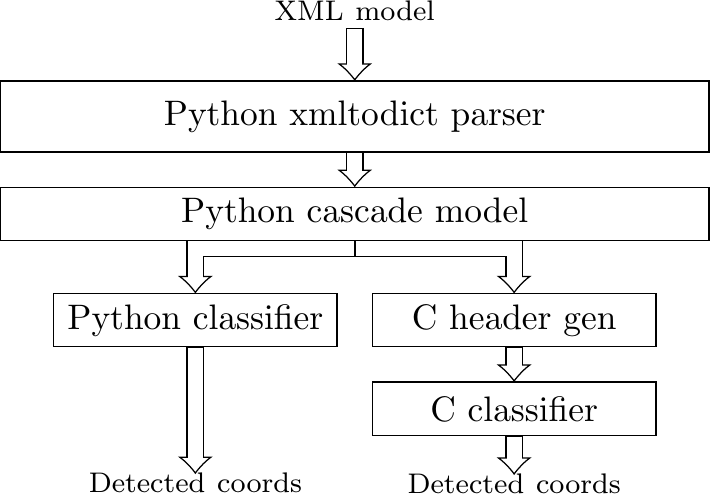
\includegraphics[width=0.9\linewidth]{bdp/sw_arch/sw_arch1.png}
  \caption{Veza Python modela sa XML modelom i C specifikacijom}
  \label{sw_arch_spec1}
\end{figure}

Na slici(\ref{sw_arch_spec1}) prikazana je struktura modela u slučaju Python i C
klasifikatora. \\

\noindent
Na ulazu se nalazi \gls{xml} model dobijen treniranjem pomoću OpenCV biblioteke opisan u sekciji
\ref{opencv_model}. \\
Parsiranje XML modela se rešava u Python-u.
Zbog velikog broja Python paketa dostupnih sa gotovim rešenjima za većinu softverskih problema, problem
parsiranja XML fajla se može rešiti korišćenjem paketa xmltodict\footnote{\url{https://pypi.org/project/xmltodict/}}. \\
\emph{Xmltodict} parsira XML fajl i skladišti ga u Python dictionary. \\
Implementirane su klase \emph{CascadeClass}, \emph{StageClass}, \emph{FeatureClass} i
\emph{RectClass}
\footnote{\texttt{\detokenize{cascade_classifier/python_model/cascade.py}}} koje
predstavljaju abstraktni Python model modela kaskadnog klasifikatora. \\

Napisana je i Python implementacija Viola-Jones algoritma koja koristi Python
model klasifikatora i koristi se kao specifikacija za izvršavanje. \\

Python model klasifikatora može da generiše \emph{C++} reprezentaciju modela
klasifikatora i sačuva ih u Header fajlove. \\
Ovim je izbegnuto parsiranje XML fajlova C++ jezikom, pošto je ovaj zadatak
mnogo jednostavnije odraditi u Python-u. \\
C++ implementacija Viola-Jones algoritma koristi ovako generisan model
klasifikatora.